\chapter{專題}

\section{语法專題}
\subsection{过去完成进行时}
\subsubsection{结构形式}
过去完成进行时由\hilight{``had been + 现在分词"}	构成,因此\hilight{无人称变化}。

\subsubsection{用法归纳}
过去完成进行时表示持续到过去某时的一个动作(可算是现在完成进行时的过去式):
\begin{itemize}
  \itemsep0em
  \item The ground was wet. \hilight{It had been raining}. 地是湿的。此前一直在下雨。
  \item At last the bus came. \hilight{I had been waiting} for half an hour. 最后公共汽车来了,我已等了半小时。
  \item She was out of breath. \hilight{She had been running}. 她气喘吁吁,她一直在跑来着。
  \item He gave up smoking last year. \hilight{He’d been smoking} for twenty years. 去年他戒烟了。他抽烟已经二十年。
\end{itemize}

过去时间可用一个时间状语表示:
\begin{itemize}
  \itemsep0em
  \item When I first met her, \hilight{she had been working} in the company for ten years. 我第一次见到她时,她在那家公司已工作十年了。
  \item I \hilight{had not been waiting} long when a taxi drew up. 我没等多久就来了一辆出租车。
  \item \hilight{She had been looking at} the parcel for some time before she realised that it was for her mother. 这包裹她\hilight{看了好一会儿}才明白这是寄给她妈的。
  \item Until / Up till then \hilight{she had been living} with her daughter. 到那时为止她一直和她女儿一起住。
\end{itemize}

但在更多情况下过去时间由另一句子表示出来,毋需加上时间状语:
\begin{itemize}
  \itemsep0em
  \item Her eyes were red. It was obvious \hilight{she had been crying}. 她眼睛红红的,显然她是哭了。
  \item Jane was annoyed. \hilight{Peter had been phoning} her every night. 简很不高兴。彼得一直每晚给打电话。
  \item He was very tired. \hilight{He had been working} all day. 他很累。他干了一整天活。
  \item She couldn’t understand him. \hilight{She hadn’t been learning} English long. 她不懂他的话。她学英语的时间还不长。
  \item I woke up — \hilight{I had been having} a bad dream. 我醒了,我做了个恶梦。
  \item She was very tired. \hilight{She had been typing} letters all day. 她很累了。她整天都在打信件。
  \item \hilight{We had been doing business} with each other for years before we quarrelled. 在吵翻之前,我们多年来在业务上一直来往。
  \item When I first met Ann, \hilight{she had been working} for Exxon for 15 years. 我第一次遇到安的时候,她已在埃克森公司干了15年了。
  \item Jenny was annoyed. \hilight{Jim had been phoning} her every night for a whole week. 詹妮生气了。整整一星期,吉姆天天晚上都给她打电话。
\end{itemize}

有时上下文可说明是谈过去的事,因此不需要时间状语:
\begin{itemize}
  \itemsep0em
  \item She had been watching TV all day. 她看了一天的电视。
  \item I had been reading your book. 我一直在看你写的书。
  \item The rain had been pouring all night. 倾盆大雨下了一整夜。
  \item We had been travelling in many countries. 我们一直在许多国家旅游。
\end{itemize}

这个时态也可用在某些从句中,这时从句的动作发生在主句的动作之前而对其有影响:
\begin{itemize}
  \itemsep0em
  \item I heard you’d been looking for me. 我听说你一直在找我。
  \item That was just the letter I had been expecting. 这正是我一直期待的信。
  \item That was exactly what we had been trying to do. 这正是我们一直想做的事。
  \item I wanted to know what had been going on. 我想知道一直在发生什么事。
  \item The drive increased the fatigue she had been feeling. 开车增加了她一直感到疲惫感觉。
  \item They said that they had been fighting for their rights all these years. 他们说这些年来他们一直在为他们的权利而斗争。
\end{itemize}

特别补充
\begin{itemize}
  \itemsep0em
  \item 凡不能用于进行时的动词均不能有这种时态,但动词want (有时还有wish) 除外。如:
  \item The boy was delighted with his new knife. He had been wanting one for a long time. 男孩对新小刀很高兴。他早就想要一把了。
  \item 过去完成进行时没有被动语态。
\end{itemize}

\section{翻譯專題}
\subsection{正確翻譯被動語態}
\begin{itemize}
  \itemsep0em
  \item He was laughed \hilight{at} by his friends. 他受到了朋友的嘲笑.
  \item Our foreign policy is supported by people all over the world. 我國的外交政策得到了全世界人民的支持.
  \item These questions will be discussed briefly. 這些問題將予以簡單討論.
  \item The boy was criticised yesterday. 這孩子昨天挨了一頓批.
  \item A police court is presided over by a magistrate, who tries the cases without a jury. 治安法庭由地方法官主持, 法官審理各種案件, 無須陪審團.
\end{itemize}

\subsection{正確翻譯過去式強調句型}
\begin{multicols}{2}
\begin{itemize}
  \itemsep0em
  \item It is generally accepted that: 普遍認為
  \item It is believed that: 據信
  \item It is well known that: 眾所周知
  \item It is learned that: 據悉
  \item It is estimated that: 據估計
  \item It must be pointed out that: 必須指出
  \item It is understood that: 不用說
  \item It cannot be denied that: 無可否認
  \item It has been proved that: 已經證明
  \item It may be confirmed that: 可以肯定
  \item It may be safely said that: 可以有把握地說
  \item It is sometimes asked that: 人們有時會問
  \item It is expected that: 人們希望
  \item It is said that: 據說
  \item It is reported that: 據報道
\end{itemize}
\end{multicols}

\subsection{正確表示时间和地點}
\subsubsection{时间}
\begin{itemize}
  \itemsep0em
  \item at + 確切時間: at seven o'clock, at noon / night / midnight, 但morning /afternoon / evening只能用``in"
  \item on + 星期 / 星期上下午 / 特别日子: on Sunday, on Sunday afternoon, on Christmas day
  \item in + 較長時間: in morning, in the summer, in 2016, in Sydney, 但noon / night只能用``at"
\end{itemize}

\subsubsection{地点}
\begin{itemize}
  \itemsep0em
  \item at, in和on 三個都是``在..."的意思, 差別只在於空間的概念.
  \item on是用在只有一面會接觸到而比較開放性的空間: stand on the ground
  \item in則是比較狹小的空間: in the room
  \item at是比較廣泛空間地點的意思, in是比較特殊具體地點的意思: I am in the build 3 at University of Wollongong 我現在在卧龙岗大学的三号楼
\end{itemize}

\begin{itemize}
  \itemsep0em
  \item at用於較明確或範圍較小的地方. 可與門牌號碼結合: at 40 Washington Street. 也可表示朝著某個方向或目標, 常與動詞搭配使用: He throw the ball at me.
  \item \textbf{at + position, place}: Wendy is at school now.
  \item \textbf{at + somewhere around us}: I am at the donut shop.
  \item \textbf{at + someone}: He is looking at me.
\end{itemize}

\begin{itemize}
  \itemsep0em
  \item in 表示``在...內", 通常指在某場所的內部. 也多用於較大的地方.
  \item \textbf{in + country / city / town / village}: I live in Sydney.
  \item \textbf{in + place inside a building}: I live in an apartment.
\end{itemize}

\begin{itemize}
  \itemsep0em
  \item on 表示``在...上", 指與含有點或面的部分接觸. 也常用於表示在街道.
  \item \textbf{on + surface, floor}: I live on the 2nd floor.
  \item \textbf{on + street name}: The department store is on Shang-Min Rd.
\end{itemize}

\begin{itemize}
  \itemsep0em
  \item at 可以單接unit, 也接具體的完整的地址, 注意英漢翻譯的時候地址從小到大顛倒!
  \item on 或 in 單接street / road
  \item in 單接suburb
  \item Arrived \hilight{in} Sydney / Arrived \hilight{at} Sydney airport.
\end{itemize}

\subsection{对女性的尊称}
\subsubsection{Miss}
维基百科中对Miss这个词来源的解释是:\textit{Originating in the 17th century, it is a contraction of mistress, which was used for all women.} Miss是mistress的缩写,mistress可以指称所有女人。(虽然mistress意为情妇,意思不是很好)

\subsubsection{Mrs. \& Ms.}
对于结了婚但并未随夫姓的女士,称呼Mrs.也是不妥的。随女权主义运动的兴起,有很多女性不愿意通过称呼体现出自己的婚姻状况(marital status),所以更倾向于被称为Ms.,这个不论是已婚还是未婚都可以用,所以为礼貌起见,第一次见到女士时,可以用这个称呼。

\subsubsection{Madam}
除了这三个平时很常用的称呼,还有其他的尊称,如madam(或者拼做madame,遵循法语里的拼法,法语字面原意为my lady),来看一下对这个词的阐释:

Madam is used in direct address, without the woman's name, especially to address whose name is not known: May I help you, madam? The male equivalent is sir.

Madam后面不用跟人名,当遇到一位不知其姓名的女士就可以这样称呼她。相对应的男性尊称为sir。

madam的缩写是ma'ma,大家很可能在电影中听到,对女王的尊称就是ma'ma。这的确是相当正式的尊称,所以平时日常生活中是不太用到的哦。

\subsubsection{Lady}
最后还有一个尊称,也是大家所熟知的:Lady,在电影和小说中我们都能看到,曾经英国贵族的女士都被尊称为Lady:

The word lady is a polite term for a woman, specifically the female equivalent to, or spouse of, a lord or gentleman, and in many contexts a term for any adult woman. Once relating specifically to women of high social class or status, over the last 300 years it has spread to embrace all adult women.

Lady是一个对女性非常客气的称呼,尤其专用于称呼地位尊贵的女性或者贵族夫人。不过在漫长的演变史中开始逐渐成为对所有女性的敬称。

其他情况下,还可以用法语词mademoiselle(等同于miss),这样的说法听起来也很高雅。

\section{詞彙專題}
\subsection{和學校有關的詞}
\begin{multicols}{2}
\begin{itemize}
  \itemsep0em
  \item \textbf{關於職位和人}:
  \begin{enumerate}
    \itemsep0em
    \item 班主任: head teacher
    \item 校長: principal / headmaster
    \item 心理咨詢師: counsellor
    \item 職業顧問: career advisor (中學里可用於幫助學生選課)
    \item 校醫: school nurse
    \item 教練: coach
  \end{enumerate}
  \item \textbf{中國特有的學歷}:
  \begin{enumerate}
    \itemsep0em
    \item 中專: Technical Secondary School
    \item 職高: Vocational Secondary School
    \item 大專: Junior College
  \end{enumerate}
  \item \textbf{不同的學生}:
  \begin{enumerate}
    \itemsep0em
    \item 寄宿 / 走讀生: boarding / day student
    \item 小學生: pupil
  \end{enumerate}
\end{itemize}
\end{multicols}

\subsection{和保險有關的詞}
\begin{multicols}{2}
\begin{itemize}
  \itemsep0em
  \item 第三方強制險: CTP (Compulsory Third Party Insurance)
  \item 綠單子: Green Slip\footnote{CTP Green Slip (NSW). Green Slip或者Compulsory Third Party insurance稱為第三方基本保險,是一種強制執行的\\汽車保險。}
  \item 建築物與屋內財產的保險: Home buildings / Home contents
  \item 收入保障: Income Protection
  \item 保單號: Policy Number
  \item 保費: premium
  \item 墊底費\footnote{墊底費,實際上是國際上大多數財產保險類公司對投保人進行理賠的時候收取損失「均攤」費用的一種通行做法。當保險投保人由於疏忽或是無可抗拒的力量,產生了財產損失並向保險公司進行索賠的時候,需要先為自己的過失造成的損失進行費用墊付;所以,Excess Fee才被稱作「墊底費」或是「打底費」,英文也稱作Deductible。}: excess fee
\end{itemize}
\end{multicols}

\subsection{和机场有关的词}
\begin{multicols}{2}
\begin{itemize}
  \itemsep0em
  \item 登机手续办理: check-in
  \item 托运的行李: checked in luggage
  \item 手提行李: carry on luggage
  \item 海关: customs
  \item 旅客出境卡: outgoing passenger card
  \item 免税店: duty-free shop
  \item 登机口: boarding gate
  \item 退税: GST refund
  \item GST: Good \& Service Tax 商品和服务税
  \item 机场传送带: reclaiming belt
  \item 承运人(公司): carrier
  \item 取行李: reclaim the baggage
  \item 靠窗位: window-seat
  \item 靠过道位: aisle-seat\footnote{aisle的s不发音}
  \item 报关物品: goods to declare
  \item 不需报关: nothing to declare
  \item 候机室: departure lounge
  \item 前往: departure to
  \item 目的地国: destination country
\end{itemize}
\end{multicols}

\subsection{和吸毒有關的詞}
\begin{multicols}{3}
\begin{itemize}
  \itemsep0em
  \item opium: 鸦片
  \item pep pill: 兴奋剂
  \item ecstasy: 迷幻劑
  \item heroin: 海洛因
  \item ice: 病毒
  \item marihuana: 大麻\footnote{大麻也称作cannabis}
  \item cocaine: 可卡因
  \item morphine: 嗎啡
  \item caffeine: 咖啡因
\end{itemize}
\end{multicols}

\begin{multicols}{2}
\begin{itemize}
  \itemsep0em
  \item drug trafficker / dealer: 毒贩
  \item drug mules: 毒骡\footnote{充当运输毒品工具的人}
  \item drug addiction: 毒瘾
  \item drug smuggler: 毒品走私贩
  \item drug rehabilitation: 戒毒
  \item drug abuse: 药物滥用
  \item drug-related crimes: 涉毒犯罪
  \item drug deal: 毒品交易
  \item drug lords: 毒枭
  \item drug possession: 持有毒品
  \item using / taking drugs: 吸毒
\end{itemize}
\end{multicols}

\subsection{和竞拍有關的詞}
\begin{multicols}{2}
\begin{itemize}
  \itemsep0em
  \item 竞价: bid, bidding
  \item 参加竞拍的人: bidder
  \item 起拍价: starting price / open bidding
  \item 成交价: hammer price / winning bid
  \item 抬高价格: bid up the price
\end{itemize}
\end{multicols}

\subsection{澳洲移民相關簽證}
\begin{itemize}
  \itemsep0em
  \item Independent Skilled Migration Scheme: 獨立技術移民方案
  \item General Skilled Migration Scheme: 一般技術移民方案
  \item Spouse / Parent Migration Scheme: 配偶 / 父母移民方案
  \item Employer / State-Government Sponsored Scheme: 雇主 / 州政府擔保方案
  \item Regional Area Sponsored Scheme: 偏遠地區擔保方案
  \item ENSOL (Employer Nomination Skill Occupation List): 雇主提名技術職業列表
  \item Visitor's Visa: 訪客簽證
  \item tourist / visitor's / student / business / working holiday (打工度假)
  \item parent / spouse / temporary skilled graduate
  \item prospective marriage visa: 預期婚姻簽證 (也叫fianc$\acute{e}$ visa: 未婚夫妻簽證)
  \item PSW (Post Study Working visa)
\end{itemize}

\subsection{和藍領職業有關的詞}
\begin{multicols}{2}
\begin{itemize}
  \itemsep0em
  \item 電工: electrician
  \item 水管工: plumber (b不發音)
  \item 木工: carpenter
  \item 石膏板(牆)工: gyprocker
  \item 磚工: bricklayer
  \item 瓷磚工: tiler
  \item (泛指)建築工人 / 承建商: builder
  \item 護工(有別於護士): nurse aid / assistant
  \item 教會醫院的護士: sister
\end{itemize}
\end{multicols}

\subsection{和銀行有關的詞}
\begin{itemize}
  \itemsep0em
  \item 西太銀行: WestPac
  \item 國民銀行: NAB (National Australia Bank)
  \item 聯邦銀行: Commonwealth Bank
  \item 澳新銀行: ANZ (Australia and New Zealand Banking Group)
\end{itemize}

\section{高端地表示倍数}
\begin{multicols}{3}
\begin{itemize}
  \itemsep0em
  \item 1: single
  \item 2: double
  \item 3: triple
  \item 4: quadruple
  \item 5: quintuple / pentuple
  \item 6: sextuple / hextuple
  \item 7: septuple
  \item 8: octuple
  \item 9: nonuple
  \item 10: decuple
  \item 11: hendecuple / undecuple
  \item 12: duodecuple
  \item 100: centuple
\end{itemize}
\end{multicols}

\subsection{宣傳冊和傳單}
\begin{itemize}
  \itemsep0em
  \item 小冊子(裝訂成冊): booklet / pamphlet / brochure
  \item 單頁傳單: flyer / leaflet
  \item 彩頁的: colour-printed
\end{itemize}

\subsection{和不同類型的房子}
\begin{multicols}{2}
\begin{itemize}
  \itemsep0em
  \item \hilight{獨棟屋: house}
  \begin{center}
    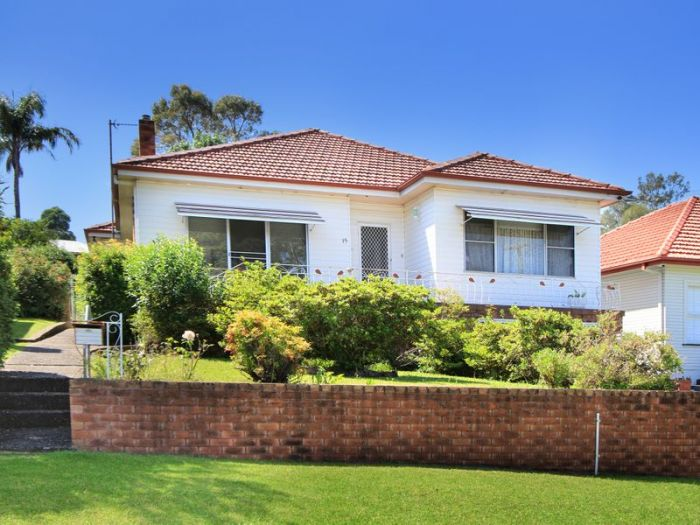
\includegraphics[scale=0.3]{pics/house}
  \end{center}
  \item 連排屋(多層): town house
  \begin{center}
    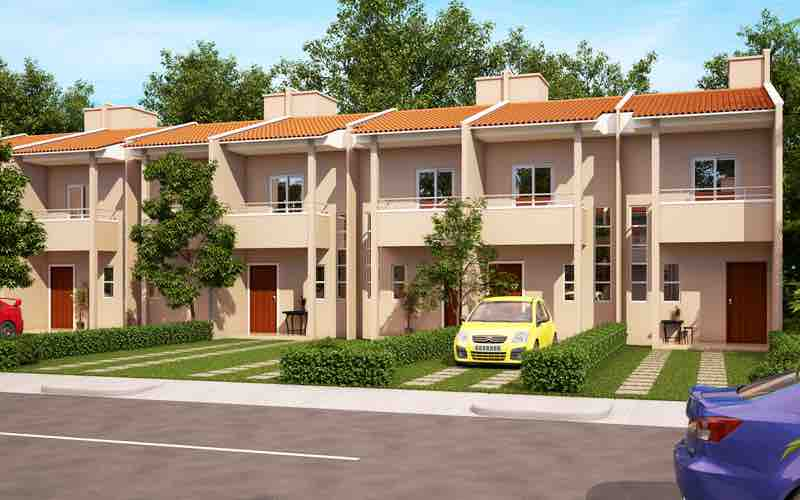
\includegraphics[scale=0.2]{pics/townhouse}
  \end{center}
  \item 後院加蓋屋 / 祖母房: granny flat
  \begin{center}
    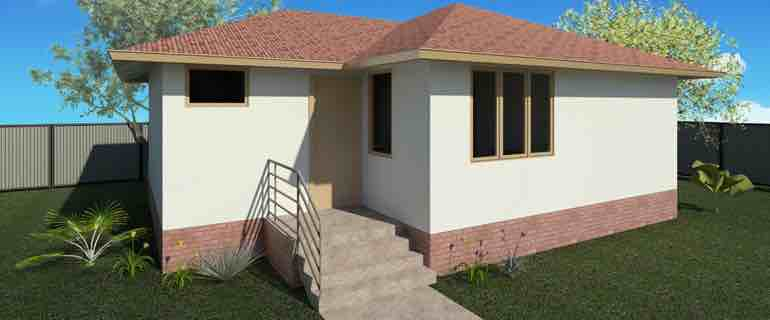
\includegraphics[scale=0.3]{pics/granny-flat}
  \end{center}
  \item \hilight{小套間: studio}
  \item 公寓: apartment
  \item 單元房: unit
\end{itemize}
\end{multicols}

\section{道德題}
\subsection{澳大利亞公眾假日}
\begin{itemize}
  \itemsep0em
  \item Australia Day: 26 January
  \item Royal Hobart Regatta: 2nd Monday in February
  \item Labour Day: 1st Monday in March
  \item Western Australia Day: 1st Monday in June
  \item Labour Day: 1st Monday in October
  \item Canberra Day: 2nd Monday in March
\end{itemize}